%%%%%%%%%%%%%%%%%%%%%%%%%%%%%%%%%%%%%%%%%%%%%%%%%%%%%%%%%%%%%%%%%%%%%%%%%%%%%%%
% Memorial para concurso público de Professor Doutor na USP.
%
% Formatação inspirada em:
% * https://tug.org/pracjourn/2008-1/mori/mori.pdf
% * https://github.com/santisoler/phd-thesis
% * https://github.com/compgeolab/dissertation-template
%%%%%%%%%%%%%%%%%%%%%%%%%%%%%%%%%%%%%%%%%%%%%%%%%%%%%%%%%%%%%%%%%%%%%%%%%%%%%%%

%%%%%%%%%%%%%%%%%%%%%%%%%%%%%%%%%%%%%%%%%%%%%%%%%%%%%%%%%%%%%%%%%%%%%%%%%%%%%%%
% Set a class and import packages
\documentclass[10pt,a4paper,oneside]{book}

% Variables
\newcommand{\Year}{2022}
\newcommand{\Title}{Memorial para concurso público - Professor Doutor em Geofísica - IAG/USP}
\newcommand{\Author}{Leonardo Uieda}
\newcommand{\Email}{Leonardo.Uieda@liverpool.ac.uk}
\newcommand{\ORCID}{0000-0001-6123-9515}
\newcommand{\ResearcherID}{G-3258-2012}
\newcommand{\GoogleScholar}{qfmPrUEAAAAJ}
\newcommand{\Lattes}{8939551682050504}

% Names for citing coauthors
\newcommand{\Me}{\textbf{Uieda, L}}
\newcommand{\Val}{Barbosa, VCF}
\newcommand{\Bi}{Oliveira Jr, VC}
\newcommand{\Paul}{Wessel, P}
\newcommand{\Joaquim}{Luis, J}
\newcommand{\Remko}{Scharroo, R}
\newcommand{\Florian}{Wobbe, F}
\newcommand{\Walter}{Smith, WHF}
\newcommand{\Dongdong}{Tian, D}
\newcommand{\Bridget}{Smith-Konter, B}
\newcommand{\Eric}{Xu, X}
\newcommand{\David}{Sandwell, DT}
\newcommand{\Carla}{Braitenberg, C}
\newcommand{\Naomi}{Ussami, N}
\newcommand{\Manoel}{D'Agrella-Filho, MS}
\newcommand{\JB}{Silva, JBC}
\newcommand{\Dai}{Sales, DP}
\newcommand{\Figura}{Melo, FF}
\newcommand{\Dio}{Carlos, DU}
\newcommand{\BragaVale}{Braga, MA}
\newcommand{\YLi}{Li, Y}
\newcommand{\Angeli}{Angeli, G}
\newcommand{\Peres}{Peres, G}
\newcommand{\Everton}{Bomfim, EP}
\newcommand{\Eder}{Molina, E}
\newcommand{\Gomes}{Gomes, AAS}
\newcommand{\Santiago}{Soler, SR}
\newcommand{\Agustina}{Pesce, A}
\newcommand{\Gimenez}{Gimenez, ME}
\newcommand{\Kristoffer}{Hallam, KAT}
\newcommand{\Guangdong}{Zhao, G}
\newcommand{\Bo}{Chen, B}
\newcommand{\JLiu}{Liu, J}
\newcommand{\LChen}{Chen, L}
\newcommand{\RGuo}{Guo, R}
\newcommand{\MKaban}{Kaban, MK}
\newcommand{\Lindsey}{Heagy, LJ}
\newcommand{\Lion}{Krischer, L}
\newcommand{\Rene}{Gassmoeller, R}
\newcommand{\Bane}{Sullivan, CB}
\newcommand{\Jens}{Klump, JF}
\newcommand{\LBarba}{Barba, LA}
\newcommand{\JBazan}{Bazan, J}
\newcommand{\JBrown}{Brown, J}
\newcommand{\RGuimera}{Guimera, RV}
\newcommand{\MGymrek}{Gymrek, M}
\newcommand{\AHanna}{Alex Hanna}
\newcommand{\KHuff}{Huff, KD}
\newcommand{\DKatz}{Katz, DS}
\newcommand{\CMadan}{Madan, CR}
\newcommand{\KMoerman}{Moerman, KM}
\newcommand{\KNiemeyer}{Niemeyer, KE}
\newcommand{\JPoulson}{Poulson, JL}
\newcommand{\PPrins}{Prins, P}
\newcommand{\KRam}{Ram, K}
\newcommand{\ARokem}{Rokem, A}
\newcommand{\Arfon}{Smith, AM}
\newcommand{\GThiruvathukal}{Thiruvathukal, GK}
\newcommand{\KThyng}{Thyng, KM}
\newcommand{\BWilson}{Wilson, BE}
\newcommand{\Yehudi}{Yehudi, Y}
\newcommand{\Remi}{Rampin, R}
\newcommand{\Hugo}{van Kemenade, H}
\newcommand{\MattTurk}{Turk, M}
\newcommand{\Shapero}{Shapero, D}
\newcommand{\Anderson}{Banihirwe, A}
\newcommand{\Leeman}{Leeman, J}
\newcommand{\JEbbing}{Ebbing, J}
\newcommand{\AGuy}{Guy, A}
\newcommand{\JFarquharson}{Farquharson, J}
\newcommand{\AKushnir}{Kushnir, A}
\newcommand{\FWadsworth}{Wadsworth, F}
\newcommand{\LPerozzi}{Perozzi, L}
\newcommand{\MWieczorek}{Wieczorek, MA}
\newcommand{\LLi}{Li, L}
\newcommand{\Ricardo}{Trindade, RIF}

\usepackage[utf8]{inputenc}
\usepackage[T1]{fontenc}
\usepackage[brazil]{babel}
\usepackage[width=150mm,top=30mm,bottom=30mm,headsep=10mm,headheight=5mm]{geometry}
\usepackage{graphicx}
\usepackage{amssymb}
\usepackage{amsmath}
\usepackage{hyperref}
% create fancy headers
\usepackage{fancyhdr}
% commands for managing dates and its formats
\usepackage{datetime2}
% improved urls with proper hyphenation
\usepackage{xurl}
% Import enumitem to customize descriptions in license.tex
\usepackage{enumitem}
% Tweak the look of captions
\usepackage{caption}
% To control the style of section titles
\usepackage{titlesec}
% Add the bibliography to the table of contents
\usepackage[nottoc,chapter]{tocbibind}
\usepackage[round,authoryear,sort]{natbib}
% Use custom apalike bibliography style
\bibliographystyle{apalike-doi}
% show dois as links on references
\usepackage{doi}
% Icon fonts (requires using xelatex or luatex)
\usepackage{fontawesome5}
\usepackage{academicons}
\usepackage{fontspec}
% Set fonts (requires compilation with xelatex)
\usepackage{fontspec}
% To make fancy text boxes
\usepackage{xcolor}
\usepackage[framemethod=tikz]{mdframed}
% For fancy and multipage tables
\usepackage{tabularx}
\usepackage{ltablex}
% To define custom environments
\usepackage{environ}
%%%%%%%%%%%%%%%%%%%%%%%%%%%%%%%%%%%%%%%%%%%%%%%%%%%%%%%%%%%%%%%%%%%%%%%%%%%%%%%

%%%%%%%%%%%%%%%%%%%%%%%%%%%%%%%%%%%%%%%%%%%%%%%%%%%%%%%%%%%%%%%%%%%%%%%%%%%%%%%
% Configuration of the document

\setmainfont[%
  Path = fonts/notoserif/,
  UprightFont = NotoSerif-Regular,
  BoldFont = NotoSerif-Bold,
  ItalicFont = NotoSerif-Italic,
  Extension = .ttf
]{NotoSerif}

% Increase the line spacing
\renewcommand{\baselinestretch}{1.5}

% Padding between the first figure and the chapter title
\newcommand{\HeroFigPad}{\vspace{-0.4cm}}

% Add a link to a DOI
\newcommand{\DOI}[1]{doi:\href{https://doi.org/#1}{#1}}

% Add a link to a GitHub repository
\newcommand{\GitHub}[1]{\faGithub{} \href{https://github.com/#1}{github.com/#1}}

% Add a link to a supplementary data
\newcommand{\Data}[1]{\aiFigshare{} dados doi:\href{https://doi.org/#1}{#1}}

% Add a link to a preprint
\newcommand{\Preprint}[1]{\aiOpenAccess{} preprint doi:\href{https://doi.org/#1}{#1}}

% Define custom colors
\definecolor{lu_gray}{gray}{0.98}
\definecolor{lu_darkgray}{gray}{0.3}
\definecolor{lu_blue}{RGB}{32, 96, 194}
\definecolor{lu_lightblue}{RGB}{238, 245, 250}
\definecolor{lu_yellow}{RGB}{255, 193, 7}
\definecolor{lu_lightyellow}{RGB}{255, 249, 230}

% Customize how Chapter headings are displayed
\titleformat{\chapter}[display]{\normalfont}{}{5pt}{\vspace{-3.5cm}\huge}[\titlerule]

% Configure captions
\captionsetup{labelfont=bf,font={small,color=lu_darkgray},skip=0pt}

% Define a fancy text box
\mdfdefinestyle{summarybox}{%
  leftline=true,
  rightline=false,
  topline=false,
  bottomline=false,
  linewidth=4pt,
  linecolor=lu_blue,
  frametitlefont=\bfseries\color{black},
  frametitlebackgroundcolor=lu_lightblue,
  frametitleaboveskip=10pt,
  frametitlebelowskip=10pt,
  frametitlerule=true,
  frametitlerulewidth=1pt,
  backgroundcolor=lu_gray,
  innertopmargin=10pt,
  innerbottommargin=15pt,
  innerleftmargin=15pt,
  innerrightmargin=15pt,
}
\newmdenv[style=summarybox]{summarybox}
\mdfdefinestyle{subsummarybox}{%
  leftline=true,
  rightline=false,
  topline=false,
  bottomline=false,
  linewidth=4pt,
  linecolor=lu_yellow,
  frametitlefont=\bfseries\color{black},
  frametitlebackgroundcolor=lu_lightyellow,
  frametitleaboveskip=10pt,
  frametitlebelowskip=10pt,
  frametitlerule=true,
  frametitlerulewidth=1pt,
  backgroundcolor=lu_gray,
  innertopmargin=10pt,
  innerbottommargin=15pt,
  innerleftmargin=15pt,
  innerrightmargin=15pt,
}
\newmdenv[style=subsummarybox]{subsummarybox}

% Define something like an fa-ul and a date list
\NewEnviron{fa-ul}{%
  \vspace{-0.4cm}
  \begin{tabularx}{\linewidth}{@{}p{0.04\linewidth}@{\hspace{0.02\linewidth}}p{0.94\linewidth}@{}}
    \BODY
  \end{tabularx}%
}
\NewEnviron{datelist}{%
  \vspace{-0.4cm}
  \begin{tabularx}{\linewidth}{@{}p{0.15\linewidth}@{\hspace{0.02\linewidth}}p{0.83\linewidth}@{}}
    \BODY
  \end{tabularx}%
}
\NewEnviron{paperlist}{%
  \vspace{-0.4cm}
  \renewcommand{\arraystretch}{1.25}
  \renewcommand{\baselinestretch}{0.5}
  \begin{tabularx}{\linewidth}{@{}p{0.08\linewidth}@{\hspace{0.02\linewidth}}p{0.9\linewidth}@{}}
    \BODY
  \end{tabularx}%
}

% Configure hyperref and add PDF metadata
\hypersetup{
    colorlinks,
    allcolors=lu_blue,
    pdftitle={\Title},
    pdfauthor={\Author},
    pdftex,
}

% make urls use the same font as every other text
\urlstyle{same}

% Configure headers and footers
\fancyhf{}
\lhead{\fontsize{10pt}{0}\selectfont\itshape \nouppercase\leftmark}
\chead{}
\rhead{\fontsize{9pt}{0}\selectfont \thepage}
\cfoot{}
\renewcommand{\headrulewidth}{0pt}
%%%%%%%%%%%%%%%%%%%%%%%%%%%%%%%%%%%%%%%%%%%%%%%%%%%%%%%%%%%%%%%%%%%%%%%%%%%%%%%

%%%%%%%%%%%%%%%%%%%%%%%%%%%%%%%%%%%%%%%%%%%%%%%%%%%%%%%%%%%%%%%%%%%%%%%%%%%%%%%
\begin{document}

\pagestyle{plain}
\frontmatter

\begin{titlepage}
  \begin{center}
    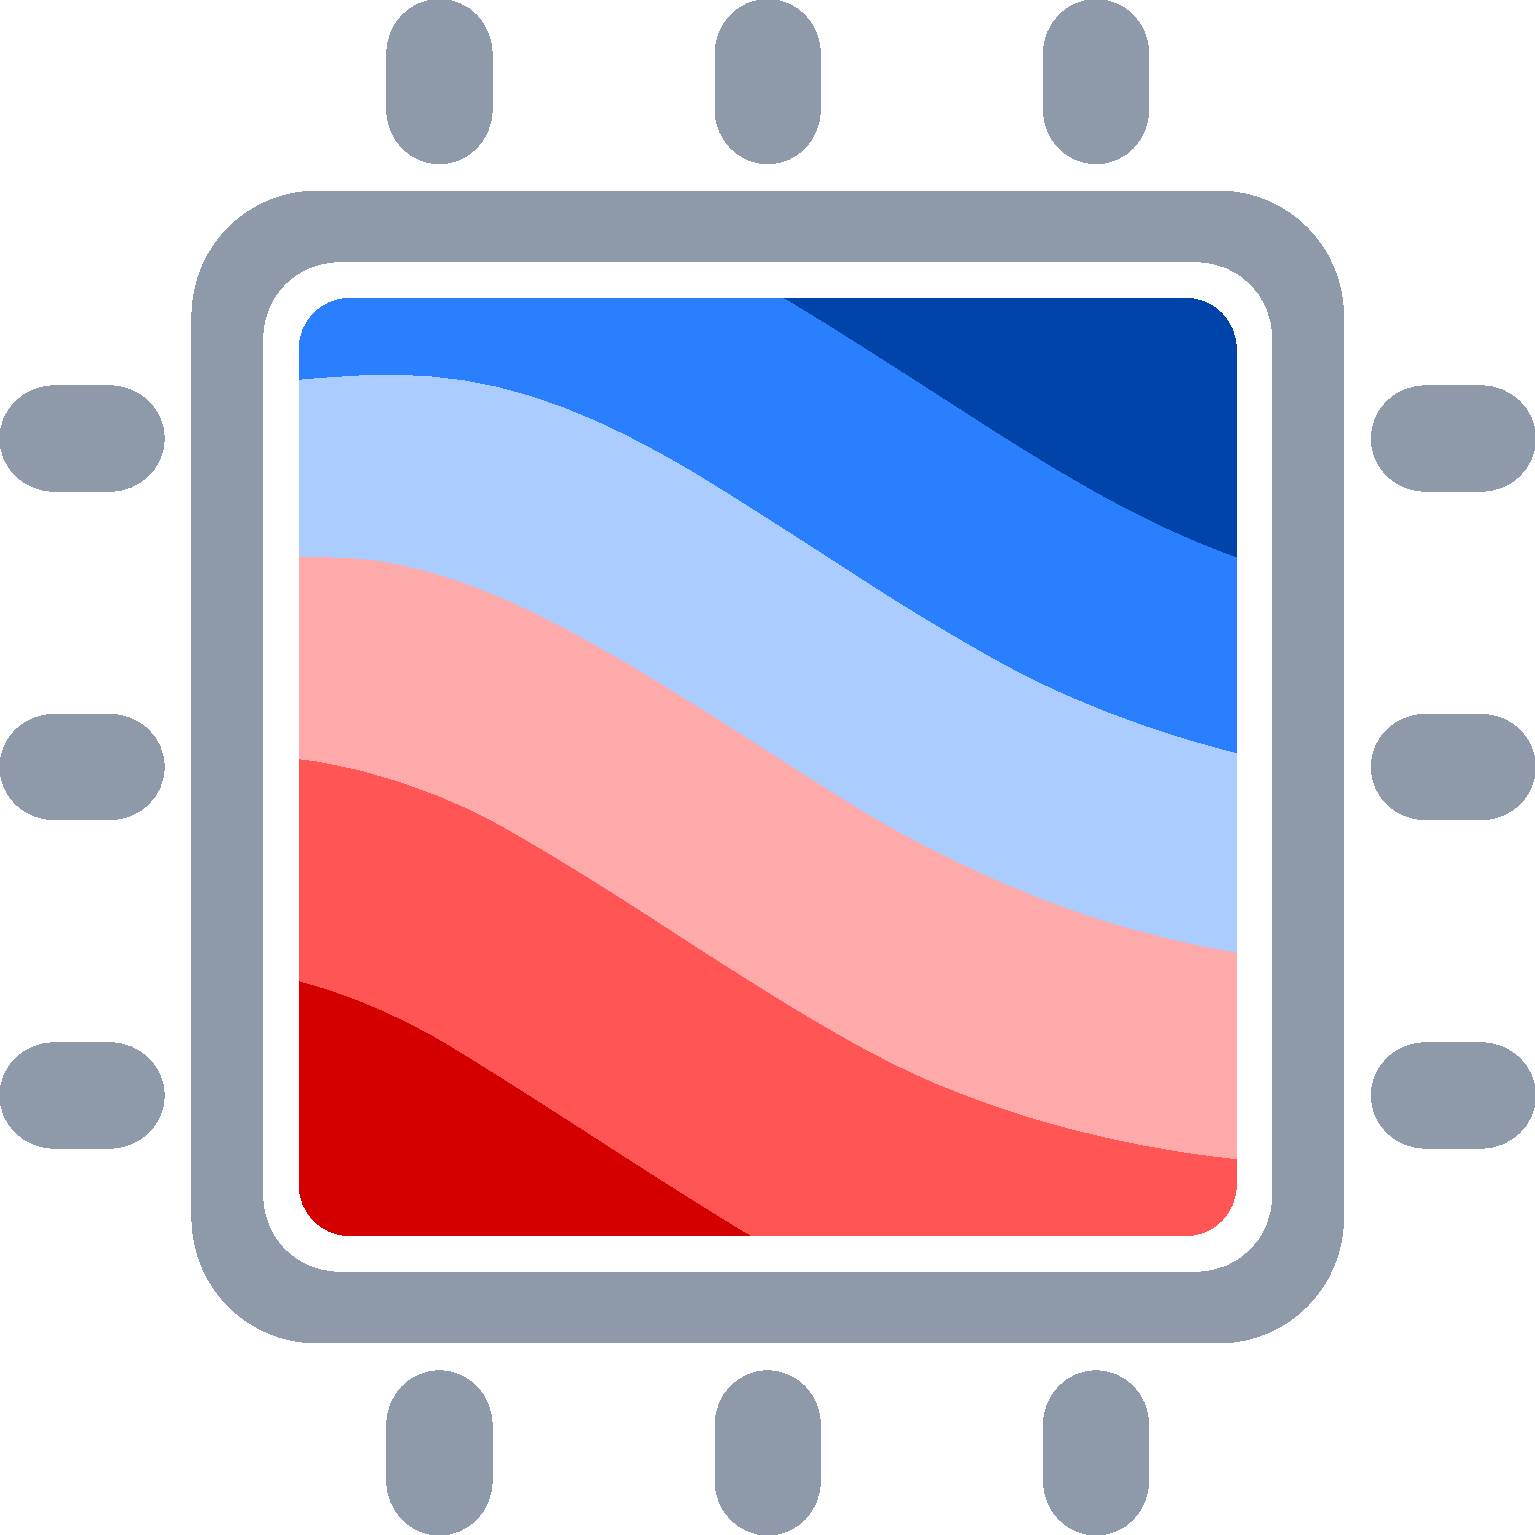
\includegraphics[height=2cm]{images/logo.pdf}
    \vspace{1cm}

    MEMORIAL PARA CONCURSO PÚBLICO

    PROFESSOR DOUTOR (RDIDP) EM MÉTODOS POTENCIAIS

    UNIVERSIDADE DE SÃO PAULO
    \vspace{4cm}

    \textbf{\LARGE \MakeUppercase{\Author{}}}
    \vspace{5cm}

    {\small
      Apresentado para concurso público de títulos e provas para cargo de

      Professor Doutor junto ao Departamento de Geofísica do

      Instituto de Astronomia, Geofísica e Ciências Atmosféricas da

      Universidade de São Paulo.
      \vspace{1cm}

      Edital ATAc-IAG/044/2022
    }
    \vfill

    \Year{}
  \end{center}
\end{titlepage}

%==============================================================================
\chapter*{Resumo}

Resumo curto.
Quem eu sou.
Principais highlights.
Sobre esse memorial (organização etc).
Meu papel no IAG.
Grande parte do texto que está na introdução do memorial antigo.

%==============================================================================
\tableofcontents

\pagestyle{fancy}
\mainmatter

%==============================================================================
\chapter{Introdução}

\begin{figure}[h]
  \HeroFigPad
  \begin{center}
    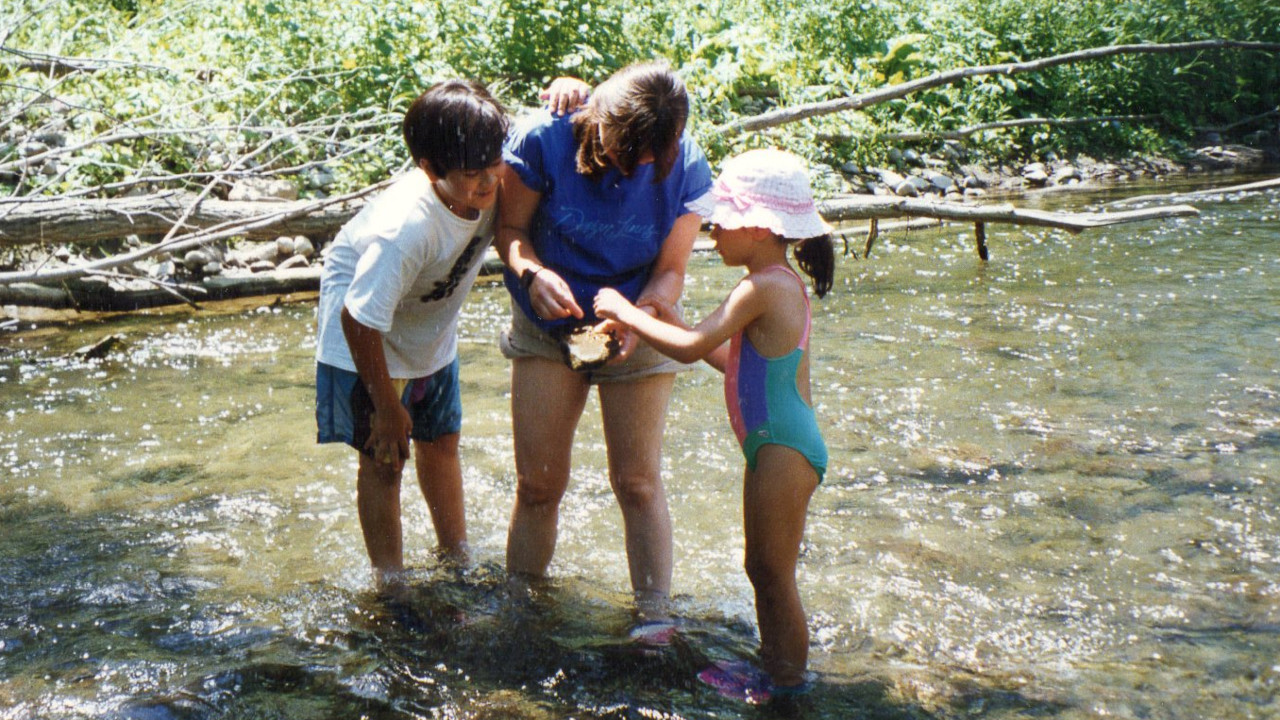
\includegraphics[width=\textwidth]{images/1997-06-ithaca-creek.jpg}
  \end{center}
  \caption{
    Minha mãe mostrando para mim e minha irmã caçula o lado inferior de uma
    pedra em um riacho, provavelmente contendo invertebrados aquáticos.
    Foto de Junho de 1997, tirada no interior do estado de Nova York, E.U.A.,
    durante o pós-doutorado de meus pais na Cornell University.
  }
  \label{fig_riacho}
\end{figure}
\begin{summarybox}[frametitle=\faInfoCircle{}\quad Informações para contato]
  \begin{fa-ul}
    \faEnvelope & email: \href{mailto:\Email}{\Email} \\
    \aiOrcid & ORCID: \href{https://orcid.org/\ORCID}{\ORCID} \\
    \aiLattes & Currículo Lattes: \href{http://lattes.cnpq.br/\Lattes}{lattes.cnpq.br/\Lattes} \\
    \aiPublonsSquare & ResearcherID: \href{https://www.webofscience.com/wos/author/rid/\ResearcherID}{\ResearcherID} \\
    \faUser & Página pessoal: \href{https://www.leouieda.com}{www.leouieda.com} \\
    \faUsers & Grupo de pesquisa: \href{https://www.compgeolab.org}{www.compgeolab.org}
  \end{fa-ul}
\end{summarybox}

\section{Influências}

Sobre meus pais e meu primeiro contato com a pesquisa e ensino superior.
A ética e dedicação eles me passaram.
A oportunidade de morar no exterior.



\section{Privilégio}

Disclaimer sobre meus privilégios.
O memorial é uma reflexão das minhas conquistas.
É importante refletir também nos privilégios que me permitiram chegar onde cheguei.
Nem tudo é mérito.
Suporte familiar.
Classe média e não tive que trabalhar para apoiar meus estudos.
Escola privada.
Oportunidade de morar fora e aprender inglês.
Brasil possui ensino superior gratuito e bolsas.
Ida para o Canada foi financiada pelos meus pais.
Muitas coisas sobre o dia a dia na academia eu já sabia por ver meus pais.
Estigma contra asiáticos é relativamente baixo, pode até ser positivo nas ciências exatas.
Sorte na escolha de curso, ano de ingresso, política a favor da ciência,
professores (Mary Lilian Lourenço, Manoel Roberto Robilotta, Alan Mitchell
Durham) e mentores (Manuel, Ricardo,
Naomi, Val, Carla, Paul), vagas na hora certa, confiança e suporte para reconhecer
opoturnidades e ir atrás.

\section{Estrutura desse memorial}

Como ficou dividido. O que tem em cada parte. Links para os capítulos. Linha do
tempo.

%==============================================================================
\chapter{Formação Acadêmica}

\begin{figure}[h]
  \HeroFigPad
  \begin{center}
    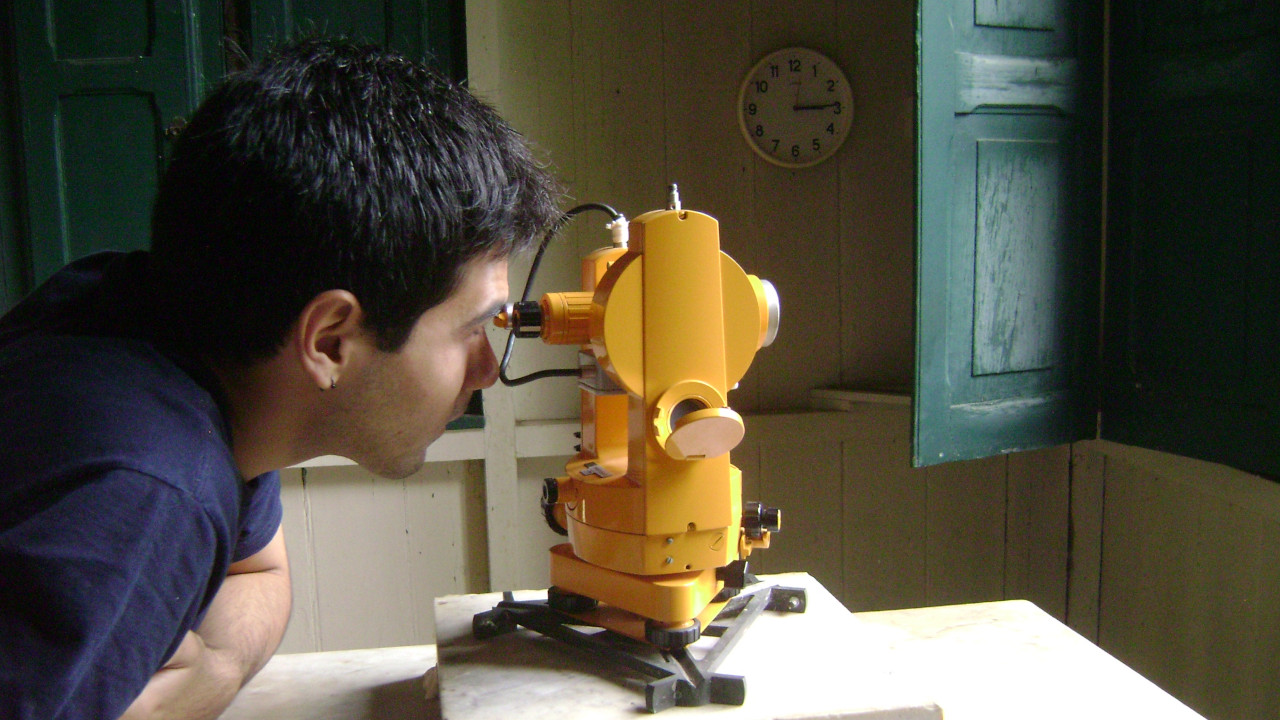
\includegraphics[width=\textwidth]{images/vassouras-geomag-observation-2012.jpg}
  \end{center}
  \caption{
    Realizando medidas da direção do campo geomagnético no observatório de
    Vassouras, RJ. A atividade foi parte de uma disciplina de instrumentação
    geofísica que cursei no mestrado do Observatório Nacional.
  }
\end{figure}
\begin{summarybox}[frametitle=\faInfoCircle{}\quad Resumo da formação acadêmica]
  \begin{datelist}
    2004--2009 & Bacharelado em Geofísica -- Universidade de São Paulo \\
    2008--2009 & \faPlane{} Intercâmbio Internacional -- York University, Canadá \\
    2010--2011 & Mestrado em Geofísica -- Observatório Nacional \\
    2011--2016 & Doutorado em Geofísica -- Observatório Nacional
  \end{datelist}
\end{summarybox}

Começa de quando ingressei na USP.
Coisas que eu aprendi, IC, TCC, campos, etc.
Turma de graduação e como isso influenciou meu pensamento.
Intercâmbio em York, geodésia, e o
Spiros Pagiatakis\footnote{\url{https://www.yorku.ca/spiros/spiros.html}}.

\section{Universidade de São Paulo}

\begin{subsummarybox}[frametitle=\faGraduationCap{}\quad Bacharelado em Geofísica]
  \begin{fa-ul}
    \faUniversity & Universidade de São Paulo \\
    \faCalendar & Fevereiro 2004 -- Novembro 2009 \\
    \faUser & Orientadora: Naomi Ussami\\
    \faInfoCircle & Trabalho de conclusão: Cálculo do tensor gradiente
    gravimétrico utilizando tesseroides \\
    \aiDoi & \DOI{10.6084/m9.figshare.963547}
  \end{fa-ul}
\end{subsummarybox}

\section{York University}

\begin{subsummarybox}[frametitle=\faPlane{}\quad Intercâmbio Internacional]
  \begin{fa-ul}
    \faUniversity & York University, Canadá\\
    \faCalendar & Agosto 2008 -- Maio 2009\\
    \faInfoCircle & Disciplinas de geodésia e posicionamento no curso de
    Engenharia Geomática.
  \end{fa-ul}
\end{subsummarybox}

\section{Observatório Nacional}

\begin{subsummarybox}[frametitle=\faGraduationCap{}\quad Mestrado em Geofísica]
  \begin{fa-ul}
    \faUniversity & Observatório Nacional \\
    \faCalendar & Fevereiro de 2010 -- Outubro de 2011 \\
    \faUser & Orientadora:  Valéria C. F. Barbosa\\
    \faInfoCircle & Dissertação: Robust 3D gravity gradient inversion by
    planting anomalous densities\\
    \aiDoi & \DOI{10.6084/m9.figshare.16882300}
  \end{fa-ul}
\end{subsummarybox}
\begin{subsummarybox}[frametitle=\faGraduationCap{}\quad Doutorado em Geofísica]
  \begin{fa-ul}
    \faUniversity & Observatório Nacional \\
    \faCalendar & Novembro de 2011 -- Abril de 2016 \\
    \faUser & Orientadora:  Valéria C. F. Barbosa\\
    \faInfoCircle & Tese Modelagem direta e inversão de campos gravitacionais em
    coordenadas esféricas \\
    \aiDoi & \DOI{10.6084/m9.figshare.16883689} \\
    \faTrophy & Ganhador do Prêmio SBGf de Melhor Tese de Doutorado (2015--2017)\footnotemark
  \end{fa-ul}
\end{subsummarybox}
\footnotetext{\url{https://sbgf.org.br/premiacoes/}}

\section{Formação complementar}

\begin{subsummarybox}[frametitle=\faGraduationCap{}\quad The Carpentries Instructor Training]
  \begin{fa-ul}
    \faUniversity & \href{https://carpentries.org/}{The Carpentries} \\
    \faCalendar & 9--10 de Julho de 2018\\
    \faInfoCircle & Habilitação para organizar e ministrar os cursos
    \textit{Software Carpentry}, \textit{Data Carpentry} e
    \textit{Library Carpentry}, incluindo treinamento em pedagogia e práticas
    de ensino de programação e ciência de dados\footnotemark{}
  \end{fa-ul}
\end{subsummarybox}
\footnotetext{\url{https://carpentries.org/instructors/\#leouieda}}
\begin{subsummarybox}[frametitle=\faGraduationCap{}\quad Postgraduate Certificate Academic Practice]
  \begin{fa-ul}
    \faUniversity & Universidade de Liverpool \\
    \faCalendar & Novembro de 2020 -- Maio de 2022 \\
    \faInfoCircle & Curso de pedagogia no ensino superior que me confere o
    título de \textit{Fellow of the Higher Education Academy}\footnotemark{}
    (número de referência PR242069)
  \end{fa-ul}
\end{subsummarybox}
\footnotetext{\url{https://www.advance-he.ac.uk/fellowship/fellowship}}

Esses foram os cursos que deram algum tipo de habilitação especial.

%==============================================================================
\chapter{Atuação Profissional}

\begin{figure}[h]
  \HeroFigPad
  \begin{center}
    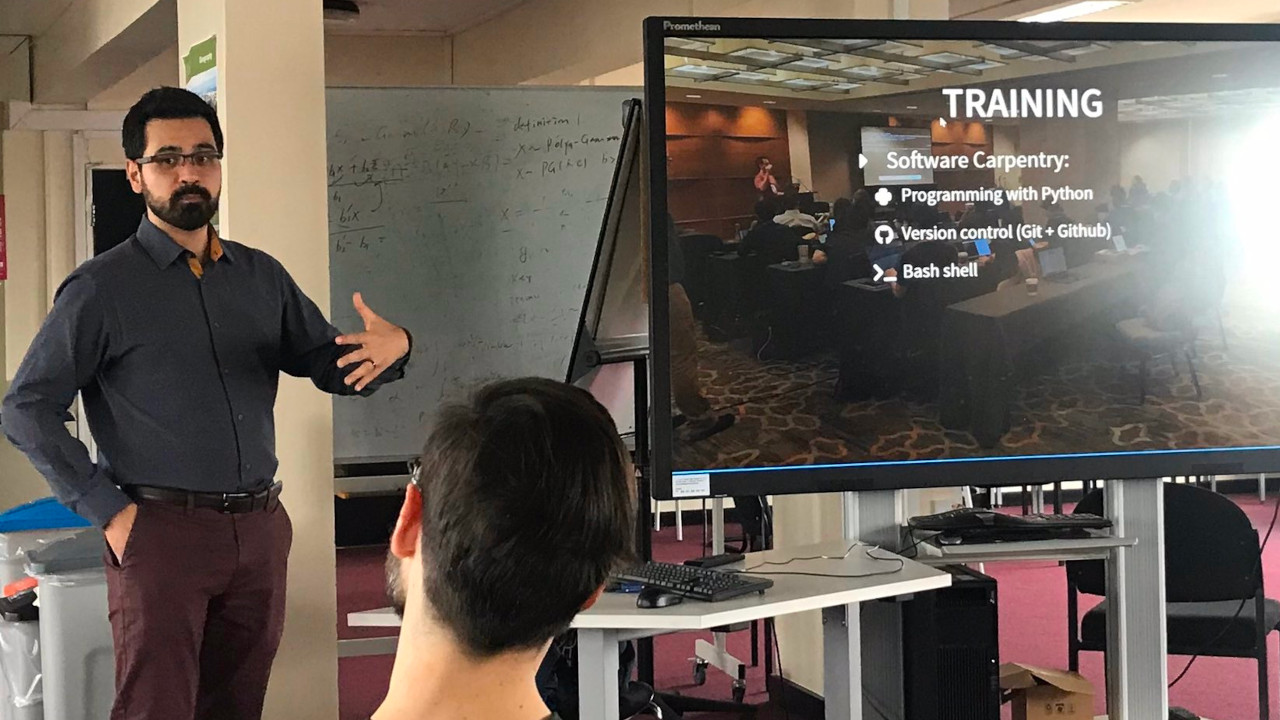
\includegraphics[width=\textwidth]{images/liverpool-gdsl.jpg}
  \end{center}
  \caption{
    Foto de uma apresentação que fiz para o \textit{Geographic Data Science
    Lab} da Universidade de Liverpool em Março de 2020. O propósito da palestra
    era me apresentar para o grupo pouco após minha chegada em Liverpool.
  }
\end{figure}
\begin{summarybox}[frametitle=\faInfoCircle{}\quad Resumo da atuação profissional]
  \begin{datelist}
    2014--2018 & Professor Assistente -- Universidade do Estado do Rio de Janeiro \\
    2017--2019 & Pesquisador Visitante -- University of Hawai`i at M\={a}noa, E.U.A. \\
    2019--atual & Lecturer (\textit{Professor Doutor}) -- University of Liverpool, Reino Unido
  \end{datelist}
\end{summarybox}

\section{Universidade do Estado do Rio de Janeiro}

\begin{subsummarybox}[frametitle=\faUniversity{}\quad Vínculo Institucional]
  \begin{fa-ul}
    \faUser & Professor Assistente \\
    \faMapMarker & Departamento de Geologia Aplicada -- Faculdade de Geologia \\
    \faCalendar & Fevereiro 2014 -- Janeiro 2018 \\
    \faTrophy & Paraninfo da turma XXX
  \end{fa-ul}
\end{subsummarybox}
\begin{subsummarybox}[frametitle=\faList{}\quad Atividades Institucionais]
  \begin{datelist}
    2014--2017 & Coordenador: Laboratório de Geofísica de Exploração (LAGEX)\\
    2014--2017 & Coordenador: Projeto Qualitec para contratação de um bolsista de nível superior para atuar no LAGEX\\
    2015--2017 & \textit{Faculty Advisor}: Capítulo Estudantil da Society of
    Exploration Geophysicists (\textit{UERJ Geophysical Society}) \\
    201X & ELEIÇÃO
  \end{datelist}
\end{subsummarybox}

SEG Chapter\footnote{\url{https://seg.org/Education/Student/Student-Chapters/Student-Chapter-Details/student-chapter-listing-details/scID/000000440245}}

Coordenação do LAGEX.

QUALITEC. Victor e Gabriela.

Capítulo SEG.

https://seg.org/Education/Student/Student-Chapters/Student-Chapter-Details/student-chapter-listing-details/scID/000000440245

Eleição


\section{University of Hawai`i at M\={a}noa}

\begin{subsummarybox}[frametitle=\faUniversity{}\quad Vínculo Institucional]
  \begin{fa-ul}
    \faUser & Pesquisador Visitante \\
    \faMapMarker & Department of Earth Sciences -- School of Ocean and Earth Science and Technology\\
    \faCalendar & Fevereiro 2017 -- Agosto 2019
  \end{fa-ul}
\end{subsummarybox}



\section{University of Liverpool}

\begin{subsummarybox}[frametitle=\faUniversity{}\quad Vínculo Institucional]
  \begin{fa-ul}
    \faUser & Lecturer (\textit{equivalente a Professor Doutor})\\
    \faMapMarker & Department of Earth, Ocean and Ecological Sciences -- School of Environmental Sciences \\
    \faCalendar & Agosto 2019 -- Presente
  \end{fa-ul}
\end{subsummarybox}
\begin{subsummarybox}[frametitle=\faList{}\quad Atividades Institucionais]
  \begin{datelist}
    2020--2022 & Comissão para avaliação do website do departamento\\
    2020--atual & Early Career Academic (ECA) Representative -- Earth Sciences\\
    2022--atual & Coordenador de curso: Bacharelado em Geofísica e Mestrado em Geologia e Geofísica
  \end{datelist}
\end{subsummarybox}

\section{Atuação na Comunidade Científica}


\begin{subsummarybox}[frametitle=\faList{}\quad Resumo das atividades]
  \begin{datelist}
    2019--2022 & \href{https://joss.theoj.org/}{Journal of Open Source Software}
    (ISSN 2475-9066): Topic Editor \\
    2019--2022 & \href{https://eartharxiv.org/}{EarthArXiv}: Advisory Council Member \\
    2022--atual & \href{https://softwareunderground.org}{Software Underground}:
             Board Member \\
    2022--atual & \href{https://www.pyopensci.org/}{pyOpenSci}:
             Advisory Committee Member
  \end{datelist}
\end{subsummarybox}

JOSS\footnote{\url{https://joss.theoj.org/about\#editors\_emeritus}}

Software Underground\footnote{\url{https://softwareunderground.org/board}}

EarthArXiv\footnote{\url{https://eartharxiv.github.io/AdvisoryCouncil.html}}

pyOpenSci\footnote{\url{https://www.pyopensci.org/our-community/\#pyopensci-working-advisory-committee}}

Revisor de periódicos\footnote{\url{https://www.webofscience.com/wos/author/rid/\ResearcherID}}:
Geophysical Journal International,
Geophysics,
Journal of Geodesy,
Pure and Applied Geophysics,
Journal of Applied Geophysics,
Geophysical Prospecting,
Central European Journal of Geosciences,
Computers and Geosciences
e
Journal of Open Source Software.

Bancas:
2022External PhD thesis examiner (Peter Haas), Christian-Albrechts-Universität zu Kiel.
2022Internal PhD thesis examiner (Yael Annemiek Engbers), University of Liverpool.
2016Internal MSc dissertation examiner (Natacha Medeiros Rocha), Universidade do Estado do Rio
de Janeiro.

Organização de eventos:

%2022 Geo+Code UK.
%2021
%Session: EOS5.3 - The evolving open-science landscape in geosciences: open data, software,
%publications and community initiatives.
%Nijzink, RC, Drost, N, Farquharson, J, Kushnir, A, Pianosi, F, Schymanski, S, Uieda, L, Wadsworth,
%F.
%EGU 2021, Vienna, Austria.
%Session: G4.3 - Acquisition and processing of gravity and magnetic field data and their
%integrative interpretation.
%Ebbing, J, Braitenberg, C, Guy, A, Kaban, MK, Uieda, L.
%EGU 2021, Vienna, Austria.
%2019
%Townhall: Update and Future Directions of the Open-Source Software Initiative.
%Uieda, L, Heagy, LJ, Krischer, L, Gassmoeller, R, Sullivan, CB.
%AGU 2019, San Francisco, USA.
%Session: NS21A - A Tour of Open-Source Software Packages for the Geosciences.
%Heagy, LJ, Gassmoeller, R, Uieda, L, Klump, JF.
%AGU 2019, San Francisco, USA.
%Townhall: The role of an open-source software initiative within the AGU.
%Heagy, LJ, Krischer, L, Uieda, L.
%AGU 2018, Washington DC, USA.


%==============================================================================
\chapter{Ciência Aberta}

\begin{figure}[h]
  \HeroFigPad
  \begin{center}
    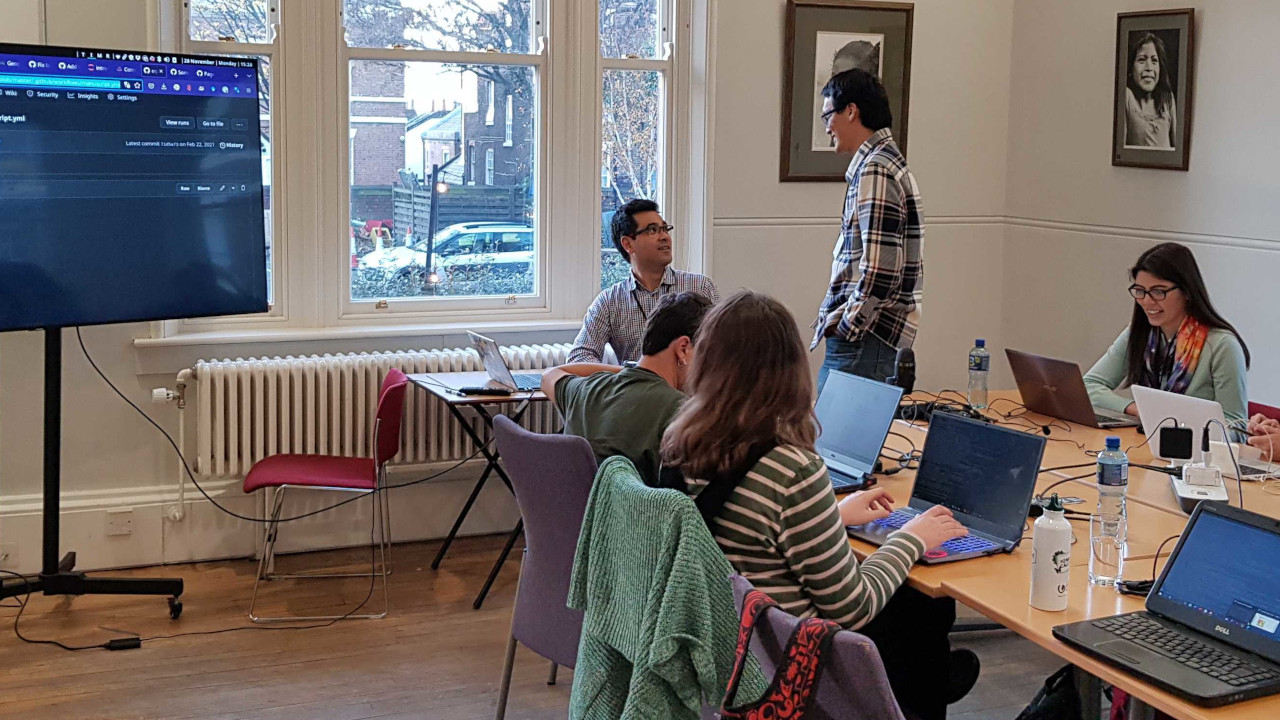
\includegraphics[width=\textwidth]{images/geopluscode.jpg}
  \end{center}
  \caption{
  }
\end{figure}
\begin{summarybox}[frametitle=\faInfoCircle{}\quad Resumo das atividades]
  \begin{fa-ul}
    \faLaptopCode & Software livre: Tesseroids, Fatiando a Terra, PyGMT \\
    \faChartBar & Dados FAIR\footnotemark{}: Tesseroids \\
    \aiOpenAccess & Acesso aberto: JOSS, EarthArXiv
  \end{fa-ul}
\end{summarybox}
\footnotetext{%
  Os princípios de dados FAIR (\textit{Findable, Accessible, Interoperable,
  Reusable}) foram estabelecidos em \citet{Wilkinson2016}.
}

Como eu abordo a pesquisa e ensino.
Computacional primeiro.
Reprodutibilidade.
Dados abertos e FAIR principles.

Materiais de ensino aberto. Citar uns artigos aqui.
SSI.
EarthArXiv.
Software Underground.

\begin{summarybox}[frametitle=\aiOpenAccess{}\quad Acesso Livre]
  \begin{fa-ul}
    \faUniversity & Universidade de São Paulo \\
    \faCalendar & Fevereiro 2004 -- Novembro 2009 \\
    \faUser & Orientadora: Naomi Ussami\\
    \aiDoi & \DOI{10.6084/m9.figshare.963547} \\
    \faInfoCircle & Trabalho de conclusão: Cálculo do tensor gradiente
    gravimétrico utilizando tesseroides
  \end{fa-ul}
\end{summarybox}

%==============================================================================
\chapter{Linhas de Pesquisa}

\begin{figure}[h]
  \HeroFigPad
  \begin{center}
    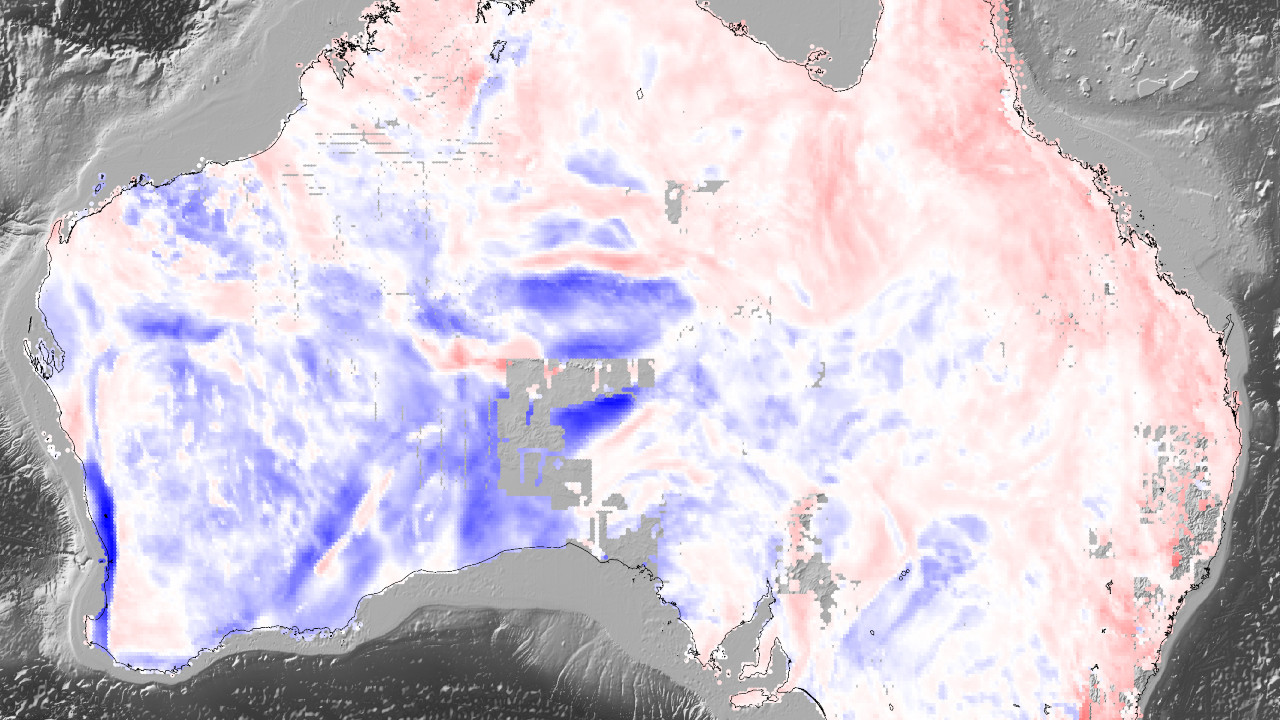
\includegraphics[width=\textwidth]{images/australia-ground-gravity-disturbance.jpg}
  \end{center}
  \caption{
    Compilação de dados terrestres de distúrbio da gravidade da Austrália.
    Distribuídos originalmente por \citet{Wynne2018}. Compilados e padronizados
    por \citet{Uieda2021}.
  }
\end{figure}
\begin{summarybox}[frametitle=\faInfoCircle{}\quad Resumo das atividades]
  \begin{fa-ul}
    \faSearchDollar & Projetos financiados pelas agências: National Science
      Foundation (E.U.A.), Royal Society (Reino Unido) e Software Sustainability
      Institute (Reino Unido)\\
    \faUserGraduate & Orientações concluídas: 11 de graduação, 1 de mestrado, 1
      co-orientação de doutorado \\
    \faFilePdf & 13 artigos publications em revistas indexadas, 3 em outras
      revistas, 11 trabalhos completos em anais de eventos \\
    \faComment & 38 apresentações de trabalho, sendo 13 dessas convidadas \\
    \aiGoogleScholarSquare & 1577 citatações nos últimos 5 anos\footnotemark{}
  \end{fa-ul}
\end{summarybox}
\footnotetext{\url{https://scholar.google.com/citations?user=qfmPrUEAAAAJ&hl=en} (acessado em 23/12/2022)}

Esse capítulo é uma reflexão da minha trajetória de pesquisa, da graduação até
minha posição atual na Universidade de Liverpool.
Ciência de impacto.
Bem social.
Grandes problemas e questões.

PINGA e CompGeoLab.

\section{Modelagem direta de campos gravitacionais em coordenadas esféricas}

Tesseroids.
Ajuda da Wild-Pfeiffer.
TCC.
Carla.
Trieste.
Discretização adaptative.
Software.
Utilização para fazer os grids do GOCE.

Projeto inicial do Santiago.
Contato com Guangdong depois de uma revisão.
Mustafa começou com a parte elipsoidal.

\begin{subsummarybox}[frametitle=\faFilePdf{}\quad Publicações nessa linha de pesquisa]
  \textbf{Artigos:}
  \begin{paperlist}
    2019 & \Santiago, \Agustina, \Gimenez, \Me.
      Gravitational field calculation in spherical coordinates using variable
      densities in depth.
      \emph{Geophysical Journal International}.
      \DOI{10.1093/gji/ggz277}.
      \GitHub{pinga-lab/tesseroid-variable-density}.
      \Preprint{10.31223/osf.io/3548g}.
      \Data{10.6084/m9.figshare.8239622}.
      \\
    ~ & \Guangdong, \Bo, \Me, \JLiu, \MKaban, \LChen, \RGuo.
      Efficient 3D large-scale forward-modeling and inversion of gravitational fields in
      spherical coordinates with application to lunar mascons.
      \emph{Journal of Geophysical Research: Solid Earth}.
      \DOI{10.1029/2019jb017691}.
      \Preprint{10.31223/osf.io/dzf9j}.
      \Data{10.6084/m9.figshare.7300523}.
      \\
    2016 & \Me, \Val, \Carla.
      Tesseroids: Forward modeling gravitational fields in spherical coordinates,
      \emph{Geophysics}, \DOI{10.1190/geo2015-0204.1}.
      \GitHub{pinga-lab/paper-tesseroids}.
  \end{paperlist}
  \noindent\textbf{Trabalhos completos em anais de eventos:}
  \begin{paperlist}
    2011 & \Me, \Everton, \Carla, \Eder.
      Optimal forward calculation method of the Marussi tensor due to a geologic
      structure at GOCE height,
      \emph{Proceedings of the 4th International GOCE User Workshop}.
      \DOI{10.6084/m9.figshare.92624}.
      \GitHub{leouieda/goce2011}.
  \end{paperlist}
\end{subsummarybox}
\begin{subsummarybox}[frametitle=\faInfoCircle{}\quad Apresentações nessa linha de pesquisa]
  \begin{paperlist}
    2010 & \Me, \Naomi, \Carla.
      Computation of the gravity gradient tensor due to topographic masses
      using tesseroids,
      \emph{AGU Meeting of the Americas},
      Foz do Iguaçu, Brazil.
      \DOI{10.6084/m9.figshare.156858}
      \\
    2008 & \Me, \Naomi.
      Utilização de tesseróides na modelagem de dados de gradiometria
      gravimétrica,
      \emph{XIII Simpósio de Iniciação Científica do IAG-USP},
      São Paulo, Brazil.
      \DOI{10.6084/m9.figshare.4779760}
  \end{paperlist}
\end{subsummarybox}



\section{Inversão 3D em métodos potenciais}

Seed e trabalhos do Dio.
Inversão do Guangdong.

\begin{subsummarybox}[frametitle=\faFilePdf{}\quad Publicações nessa linha de pesquisa]
  \textbf{Artigos:}
  \begin{paperlist}
  \end{paperlist}
  \noindent\textbf{Trabalhos completos em anais de eventos:}
  \begin{paperlist}
  \end{paperlist}
\end{subsummarybox}
\begin{subsummarybox}[frametitle=\faInfoCircle{}\quad Apresentações nessa linha de pesquisa]
  \begin{paperlist}
  \end{paperlist}
\end{subsummarybox}



\section{Determinação da espessura crustal através de distúrbios da gravidade}

Inversão Moho. Citações e utilização do software em outras áreas.

\begin{subsummarybox}[frametitle=\faFilePdf{}\quad Publicações nessa linha de pesquisa]
  \textbf{Artigos:}
  \begin{paperlist}
  \end{paperlist}
\end{subsummarybox}
\begin{subsummarybox}[frametitle=\faInfoCircle{}\quad Apresentações nessa linha de pesquisa]
  \begin{paperlist}
  \end{paperlist}
\end{subsummarybox}


\section{Deconvolução de Euler}

Trabalho do Felipe Melo.
Tutorial na TLE.
Projeto do Lottie.
Projeto do Gelson.

\begin{subsummarybox}[frametitle=\faFilePdf{}\quad Publicações nessa linha de pesquisa]
  \textbf{Artigos:}
  \begin{paperlist}
  \end{paperlist}
  \noindent\textbf{Trabalhos completos em anais de eventos:}
  \begin{paperlist}
  \end{paperlist}
\end{subsummarybox}
\begin{subsummarybox}[frametitle=\faInfoCircle{}\quad Apresentações nessa linha de pesquisa]
  \begin{paperlist}
  \end{paperlist}
\end{subsummarybox}


\section{Camada equivalente para processamento de dados gravimétricos e magnetométricos}

PEL.
Gradient boosting.
Validação cruzada em blocos.
Trazendo coisas da aprendizagem de máquinas.

Projeto da India para juntar dados da Antártica.
Projeto do Hamed para juntar grav australia.

\begin{subsummarybox}[frametitle=\faFilePdf{}\quad Publicações nessa linha de pesquisa]
  \textbf{Artigos:}
  \begin{paperlist}
  \end{paperlist}
  \noindent\textbf{Trabalhos completos em anais de eventos:}
  \begin{paperlist}
  \end{paperlist}
\end{subsummarybox}
\begin{subsummarybox}[frametitle=\faInfoCircle{}\quad Apresentações nessa linha de pesquisa]
  \begin{paperlist}
  \end{paperlist}
\end{subsummarybox}

\section{Interpolação de dados geofísicos}

Verde e interpolação de GPS com o Sandwell.


\section{Desenvolvimento de software científico}

Os códigos que possibilitam a pesquisa.
Tesseroids, Fatiando, Verde, Pooch, PyGMT, GMT.
Projetos da NSF e SSI.


\section{Modelagem de dados de microscopia magnética}

Projeto do Gelson.
Junta com o paper da Dai (colocar aqui).
Financiamento da Royal Society.
Voltando à paleomag depois da primeira IC.


\section{Determinação do fluxo geotermal Antártico através de dados magnetométricos}

Projeto da India que tá começando junto com o Bi.
Colaboração com o pessoal da BAS e o Lu Li.
Usar a compilação de dados produzida com camada equivalente para fazer uma
inversão usando tesseroides.


%==============================================================================
\chapter{Experiência em Ensino}

\begin{figure}[h]
  \HeroFigPad
  \begin{center}
    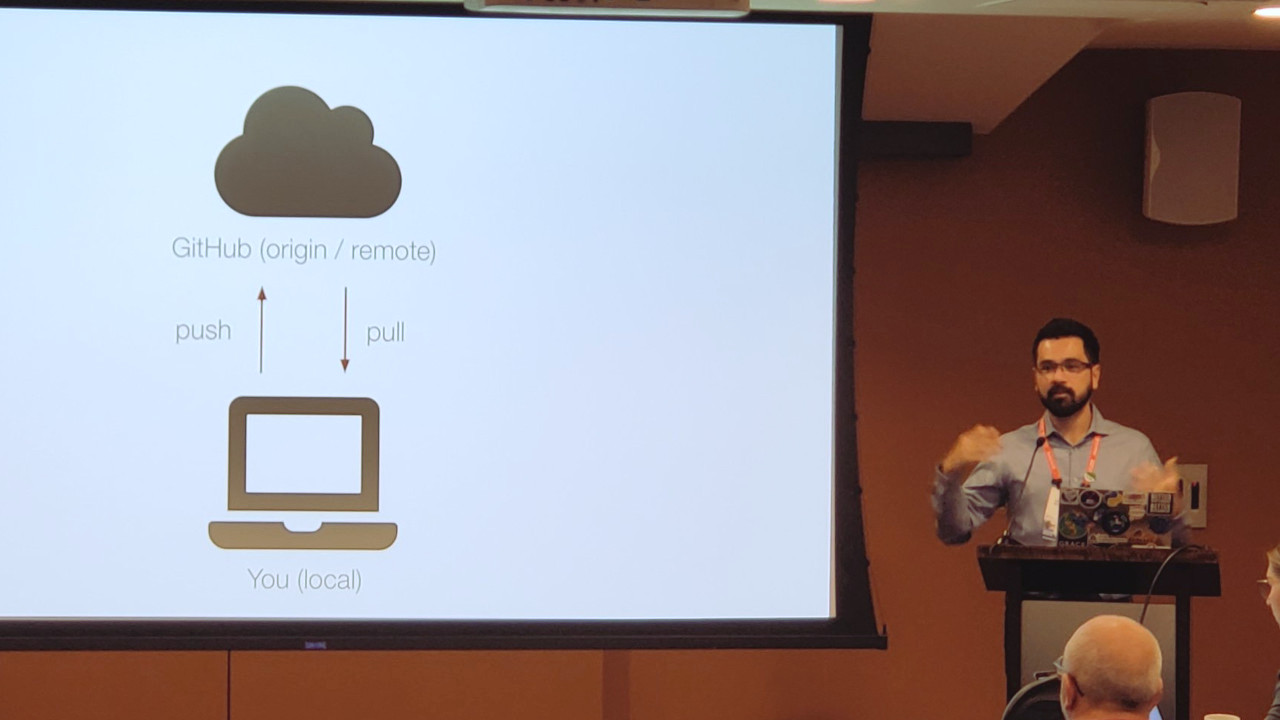
\includegraphics[width=\textwidth]{images/agu-2019-git-lesson.jpg}
  \end{center}
  \caption{
    Bla
  }
\end{figure}
\begin{summarybox}[frametitle=\faChalkboardTeacher{}\quad Resumo da Experiência de Ensino]
  \begin{fa-ul}
    \faChalkboardTeacher & X disciplinas de graduação ministradas em Y instituições \\
    \faClock & X cursos de curta duração ministrados internacionalmente \\
    \faCheckCircle & Habilitação em pedagogia e técnicas de ensino aplicadas ao ensino superior
  \end{fa-ul}
\end{summarybox}

Ensino é a parte que eu mais gosto.
Como eu abordo o ensino.
Citar artigos de pedagogia.
Figura do notebook de ondas sísmicas.
Ensino guiando a pesquisa (imagem do Havaí e trabalho do Gelson).

Crise na geociêcias.
Fenômeno global citar trabalhos nos EUA e Inglaterra.
Qual é o papel da geofísica além do petróleo.
Ciência de dados.
Aplicações ambientais.
Importância de conceitos de programação para ser cidadão informado no século XXI.

\section{Cursos de curta duração}

\begin{subsummarybox}[frametitle=\faClock{}\quad Cursos e workshops ministrados]
\end{subsummarybox}

Primeira experiência na USP.
Escolas de verão no Brasil.
Software Carpentry.
AGU.
GMT e GMTSAR.
Transform.

\section{Disciplinas de graduação}

\begin{subsummarybox}[frametitle=\faClock{}\quad Disciplias ministrados]
\end{subsummarybox}

Matérias que eu criei.
Material didático.
Paraninfo da turma.
Disciplinas de campo.

PGCAP.
Disciplinas de campo.
Matérias criadas em Liverpool.
Machine learning.
Environmental Data Science em todos os cursos.
Coordenação do curso.


%==============================================================================
\chapter{Conclusão}

Repete resumo dos principais pontos.
Termina com o que eu pretendo conquistar no futuro.

%==============================================================================
\backmatter
%\phantomsection  % use phantomsection to fix bibliography href in the toc
\bibliography{references}

\end{document}
